
\documentclass[border=10pt, 12pt]{standalone}
\usepackage[svgnames]{xcolor}
\usepackage{amsmath}
\usepackage{pgfplots}
\pgfplotsset{compat=newest}
\usepackage[sfdefault]{FiraSans}
\usepackage{FiraMono}
\renewcommand*\familydefault{\sfdefault}
\begin{document}
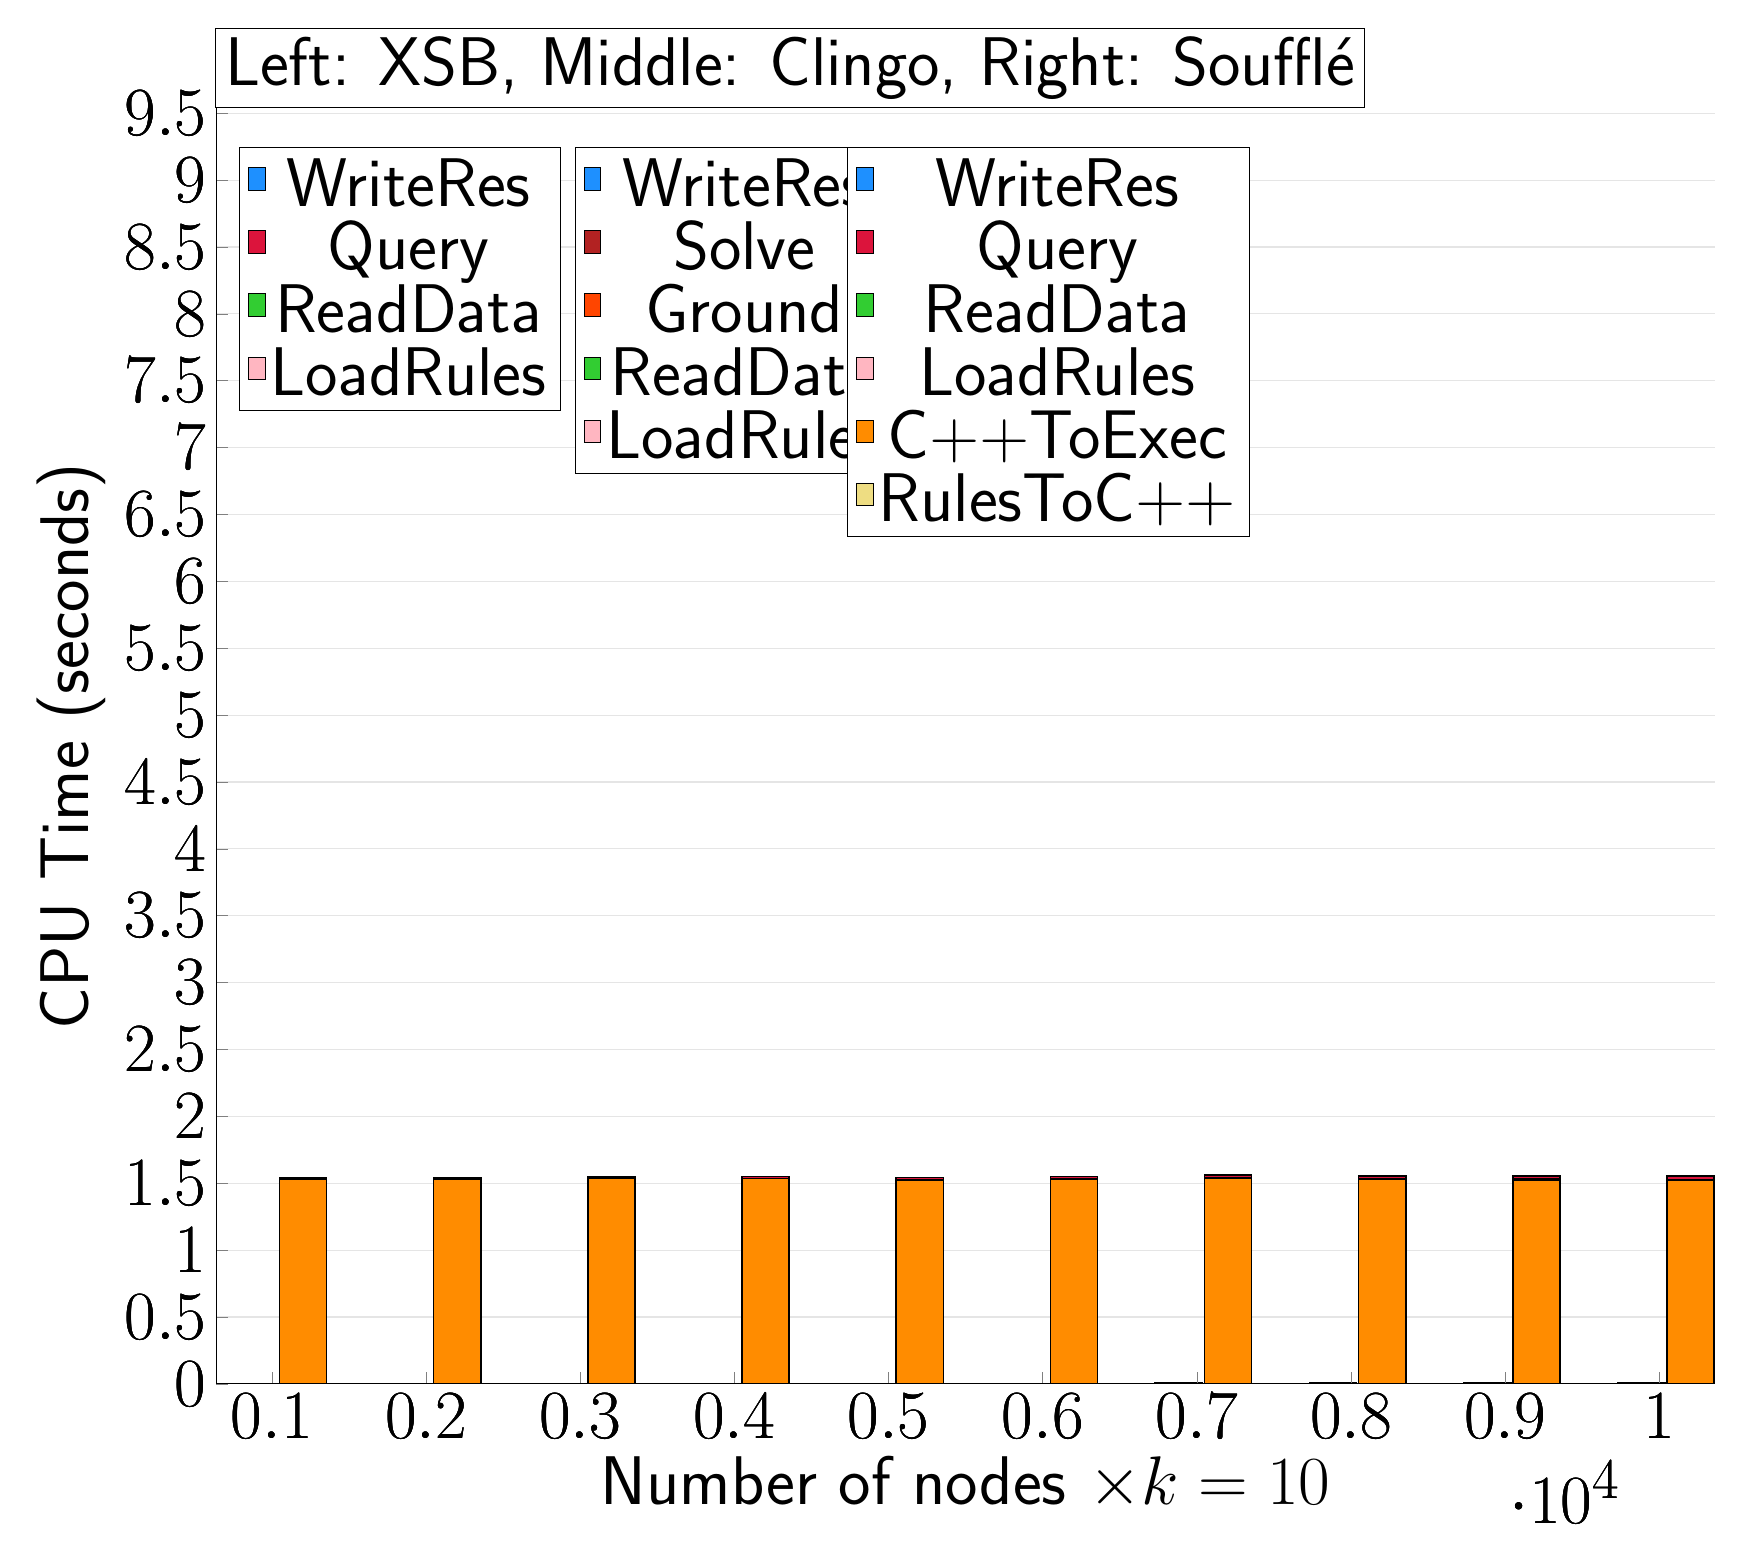
\begin{tikzpicture}
                        \begin{axis}[bar shift=-24.3pt, 
   ybar stacked,
   width=1.7\textwidth,
   bar width=0.6cm,
   ymajorgrids, tick align=inside,
   major grid style={draw=gray!20},
   xtick=data,
   ymin=0, ymax=9.536,
   axis x line*=bottom,
   axis y line*=left,
   enlarge x limits=0.04,
   legend style={
       at={(0.23, 0.97)},
       anchor=north east,
       legend columns=1,
       font=\Huge,
   },
   ylabel={CPU Time (seconds)},
   xlabel={Number of nodes $\times k=10$},
   label style={font=\Huge},
   tick label style={font=\Huge},
]
\addlegendimage{fill=DodgerBlue, draw=black, line width=0.2pt}
\addlegendentry{WriteRes}
\addlegendimage{fill=Crimson, draw=black, line width=0.2pt}
\addlegendentry{Query}
\addlegendimage{fill=LimeGreen, draw=black, line width=0.2pt}
\addlegendentry{ReadData}
\addlegendimage{fill=LightPink, draw=black, line width=0.2pt}
\addlegendentry{LoadRules}
\addplot +[fill=LightPink, draw=black, line width=0.55pt] coordinates {
(1000, 0.0005544)
(2000, 0.0005538000000000007)
(3000, 0.000553)
(4000, 0.0005567999999999999)
(5000, 0.0005568000000000001)
(6000, 0.0005508000000000004)
(7000, 0.0005692)
(8000, 0.0005552000000000005)
(9000, 0.0005699999999999997)
(10000, 0.000552)
};
\addplot +[fill=LimeGreen, draw=black, line width=0.55pt] coordinates {
(1000, 0.0002092000000000004)
(2000, 0.0002867999999999998)
(3000, 0.0003673999999999996)
(4000, 0.0004415999999999998)
(5000, 0.0005257999999999999)
(6000, 0.0006041999999999995)
(7000, 0.0006799999999999995)
(8000, 0.0007505999999999998)
(9000, 0.0008135999999999999)
(10000, 0.0009410000000000002)
};
\addplot +[fill=Crimson, draw=black, line width=0.55pt] coordinates {
(1000, 1.1399999999999638e-05)
(2000, 1.219999999999974e-05)
(3000, 1.2000000000000241e-05)
(4000, 1.180000000000004e-05)
(5000, 1.180000000000004e-05)
(6000, 1.200000000000024e-05)
(7000, 1.3200000000000399e-05)
(8000, 1.1599999999999838e-05)
(9000, 1.239999999999958e-05)
(10000, 1.219999999999972e-05)
};
\addplot +[fill=DodgerBlue, draw=black, line width=0.55pt] coordinates {
(1000, 6.540000000000014e-05)
(2000, 6.360000000000011e-05)
(3000, 6.19999999999995e-05)
(4000, 6.699999999999999e-05)
(5000, 6.479999999999991e-05)
(6000, 6.379999999999959e-05)
(7000, 6.339999999999989e-05)
(8000, 6.539999999999946e-05)
(9000, 6.300000000000054e-05)
(10000, 6.30000000000002e-05)
};
\end{axis}

\begin{axis}[bar shift=-6.5pt, 
   ybar stacked,
   width=1.7\textwidth,
   bar width=0.6cm,
   ymajorgrids, tick align=inside,
   major grid style={draw=none},
   xtick=data,
   ymin=0, ymax=9.536,
   axis x line*=none,
   axis y line*=none,
   enlarge x limits=0.04,
   legend style={
       at={(0.454, 0.97)},
       anchor=north east,
       legend columns=1,
       font=\Huge,
   },
   label style={font=\Huge},
   tick label style={font=\Huge},
]
\addlegendimage{fill=DodgerBlue, draw=black, line width=0.2pt}
\addlegendentry{WriteRes}
\addlegendimage{fill=FireBrick, draw=black, line width=0.2pt}
\addlegendentry{Solve}
\addlegendimage{fill=OrangeRed, draw=black, line width=0.2pt}
\addlegendentry{Ground}
\addlegendimage{fill=LimeGreen, draw=black, line width=0.2pt}
\addlegendentry{ReadData}
\addlegendimage{fill=LightPink, draw=black, line width=0.2pt}
\addlegendentry{LoadRules}
\addplot +[fill=LightPink, draw=black, line width=0.55pt] coordinates {
(1000, 0.0)
(2000, 0.0)
(3000, 0.0)
(4000, 0.0)
(5000, 0.0)
(6000, 0.0)
(7000, 0.0)
(8000, 0.0)
(9000, 0.0)
(10000, 0.0)
};
\addplot +[fill=LimeGreen, draw=black, line width=0.55pt] coordinates {
(1000, 0.0)
(2000, 0.0)
(3000, 0.0)
(4000, 0.0)
(5000, 0.0)
(6000, 0.0)
(7000, 0.0)
(8000, 0.0)
(9000, 0.0)
(10000, 0.0)
};
\addplot +[fill=OrangeRed, draw=black, line width=0.55pt] coordinates {
(1000, 0.0)
(2000, 0.0)
(3000, 0.0)
(4000, 0.0)
(5000, 0.0)
(6000, 0.0020000000000000018)
(7000, 0.006000000000000005)
(8000, 0.0040000000000000036)
(9000, 0.006000000000000005)
(10000, 0.010000000000000009)
};
\addplot +[fill=FireBrick, draw=black, line width=0.55pt] coordinates {
(1000, 0.0)
(2000, 0.0)
(3000, 0.0)
(4000, 0.0)
(5000, 0.0)
(6000, 0.0)
(7000, 0.0)
(8000, 0.0020000000000000018)
(9000, 0.0020000000000000005)
(10000, 0.0)
};
\addplot +[fill=DodgerBlue, draw=black, line width=0.55pt] coordinates {
(1000, 0.0)
(2000, 0.0)
(3000, 0.0)
(4000, 0.0)
(5000, 0.0)
(6000, 0.0)
(7000, 0.0)
(8000, -0.0020000000000000018)
(9000, -0.0020000000000000005)
(10000, 0.0)
};
\end{axis}

\begin{axis}[bar shift=11.3pt, 
   ybar stacked,
   width=1.7\textwidth,
   bar width=0.6cm,
   ymajorgrids, tick align=inside,
   major grid style={draw=none},
   xtick=data,
   ymin=0, ymax=9.536,
   axis x line*=none,
   axis y line*=none,
   enlarge x limits=0.04,
   legend style={
       at={(0.69, 0.97)},
       anchor=north east,
       legend columns=1,
       font=\Huge,
   },
   label style={font=\Huge},
   tick label style={font=\Huge},
]
\addlegendimage{fill=DodgerBlue, draw=black, line width=0.2pt}
\addlegendentry{WriteRes}
\addlegendimage{fill=Crimson, draw=black, line width=0.2pt}
\addlegendentry{Query}
\addlegendimage{fill=LimeGreen, draw=black, line width=0.2pt}
\addlegendentry{ReadData}
\addlegendimage{fill=LightPink, draw=black, line width=0.2pt}
\addlegendentry{LoadRules}
\addlegendimage{fill=DarkOrange, draw=black, line width=0.2pt}
\addlegendentry{C++ToExec}
\addlegendimage{fill=LightGoldenrod, draw=black, line width=0.2pt}
\addlegendentry{RulesToC++}
\addplot +[fill=LightGoldenrod, draw=black, line width=0.55pt] coordinates {
(1000, 0.0)
(2000, 0.0)
(3000, 0.0020000000000000005)
(4000, 0.0)
(5000, 0.0)
(6000, 0.0)
(7000, 0.0)
(8000, 0.0020000000000000018)
(9000, 0.0)
(10000, 0.0)
};
\addplot +[fill=DarkOrange, draw=black, line width=0.55pt] coordinates {
(1000, 1.5320000000000003)
(2000, 1.528)
(3000, 1.532)
(4000, 1.5340000000000003)
(5000, 1.5240000000000002)
(6000, 1.53)
(7000, 1.536)
(8000, 1.526)
(9000, 1.526)
(10000, 1.52)
};
\addplot +[fill=LightPink, draw=black, line width=0.55pt] coordinates {
(1000, 0.0001618)
(2000, 0.0001608)
(3000, 0.0001568)
(4000, 0.00016759999999999998)
(5000, 0.0001682)
(6000, 0.0001554)
(7000, 0.0001708)
(8000, 0.000157)
(9000, 0.00015460000000000002)
(10000, 0.000156)
};
\addplot +[fill=LimeGreen, draw=black, line width=0.55pt] coordinates {
(1000, 0.0009177999999999999)
(2000, 0.0012559999999999997)
(3000, 0.0015476)
(4000, 0.002077)
(5000, 0.0024763999999999997)
(6000, 0.0027406)
(7000, 0.0031945999999999997)
(8000, 0.0033938)
(9000, 0.0038921999999999997)
(10000, 0.0042254)
};
\addplot +[fill=Crimson, draw=black, line width=0.55pt] coordinates {
(1000, 0.0043354)
(2000, 0.007401600000000001)
(3000, 0.009592)
(4000, 0.013355200000000001)
(5000, 0.0163014)
(6000, 0.018557200000000003)
(7000, 0.021029799999999998)
(8000, 0.0232192)
(9000, 0.0251688)
(10000, 0.0277614)
};
\addplot +[fill=DodgerBlue, draw=black, line width=0.55pt] coordinates {
(1000, 0.0003888)
(2000, 0.00032639999999999996)
(3000, 0.000234)
(4000, 0.0002496)
(5000, 0.0002896)
(6000, 0.0002904)
(7000, 0.000245)
(8000, 0.000266)
(9000, 0.0002532)
(10000, 0.000256)
};
\end{axis}


\node[anchor=south, draw, fill=white] at (rel axis cs:0.42,1) {\Huge Left: XSB, Middle: Clingo, Right: Soufflé};
\end{tikzpicture}
\end{document}
                    